
\chapter{Examples}
\label{chap:examples}

\section{teste}
\subsection{teste}
\subsubsection{teste}
\begin{algorithm2e}
\caption{Gauss-Seidel Algorithm}\label{alg:gauss-seidel}
\KwIn
{%
scalar $\epsilon$,
matrix $\mathbf{A} = (a_{ij})$,
vector $\vec{b}$
and initial vector $\vec{x}^{(0)}$
}
\For{$k\leftarrow 1$ \KwTo maximum iterations}
{
\For{$i\leftarrow 1$ \KwTo $n$}
{
$
x_i^{(k)} =
\frac
{
b_i-\sum_{j=1}^{i-1}a_{ij}x_j^{(k)}
-\sum_{j=i+1}^{n}a_{ij}x_j^{(k-1)}
}%
{a_{ii}}
$\;
}
\If{$\lvert\vec{x}^{(k)}-\vec{x}^{(k-1)}\rvert < \epsilon$}
{Stop}
}
\end{algorithm2e}

% \begin{table}[H]
%   \centering
%   \caption{table}
%   \begin{tabular}{cc}
%     \label{tab:tab1}
%     \hypertarget{tab:1}{}
%     Transição&Significado\\
%     \hline \\
%     \hyperlink{partialNet:t1}{\hypertarget{partialTable:t1}{$t_{1}$}}&Test\\
%     \hyperlink{partialNet:p1}{\hypertarget{partialTable:p1}{$p_{1}$}}&balbalbal\\
%     \hyperlink{partialNet:p0m2}{\hypertarget{partialTable:p0m2}{$p_{0}$}}&balbalbal
%   \end{tabular}
% \end{table}

% \newpage
% \begin{figure}[h]
%   \centering
%   \begin{tikzpicture}[>=latex',line join=bevel,]
%%
\node (p0m2) at (27.0bp,18.0bp) [draw,ellipse,place, tokens=2, label=above:, label=left:\hyperlink{partialTable:p0m2}{\hypertarget{partialNet:p0m2}{$p_{0}$}},rotate=90] {};
  \node (tt1) at (114.0bp,18.0bp) [draw,ellipse,timedtransition, label=above:, label=left:\hyperlink{partialTable:tt1}{\hypertarget{partialNet:tt1}{$t_{1}$}},rotate=90] {};
  \node (ep1) at (185.0bp,18.0bp) [draw,ellipse,extPlace, label=above:, label=left:\hyperlink{partialNet:p1}{$p_{1}$},rotate=90] {};
  \draw [-Latex,inhibitor] (p0m2) ..controls (54.05bp,18.0bp) and (76.966bp,18.0bp)  .. (tt1);
  \definecolor{strokecol}{rgb}{0.0,0.0,0.0};
  \pgfsetstrokecolor{strokecol}
  \draw (70.5bp,27.0bp) node {3};
  \draw [-Latex] (tt1) ..controls (141.25bp,18.0bp) and (147.94bp,18.0bp)  .. (ep1);
%
\end{tikzpicture}

%   \caption{example }
%   \label{fig:example}
% \end{figure}

% \newpage
% \begin{figure}[h]
%   \centering
%   \begin{tikzpicture}[>=latex',line join=bevel,]
%%
\node (et1) at (27.0bp,18.0bp) [draw,ellipse,extTransition, label=above:, label=left:\hyperlink{partialNet:t1}{$t_{1}$},rotate=90] {};
  \node (p1) at (95.0bp,18.0bp) [draw,ellipse,place, label=above:, label=left:\hyperlink{partialTable:p1}{\hypertarget{partialNet:p1}{$p_{1}$}},rotate=90] {};
  \draw [-Latex] (et1) ..controls (54.266bp,18.0bp) and (57.727bp,18.0bp)  .. (p1);
%
\end{tikzpicture}

%   \caption{example }
%   \label{fig:example}
% \end{figure}

% \newpage

% \begin{figure}[H]
%   \centering
%   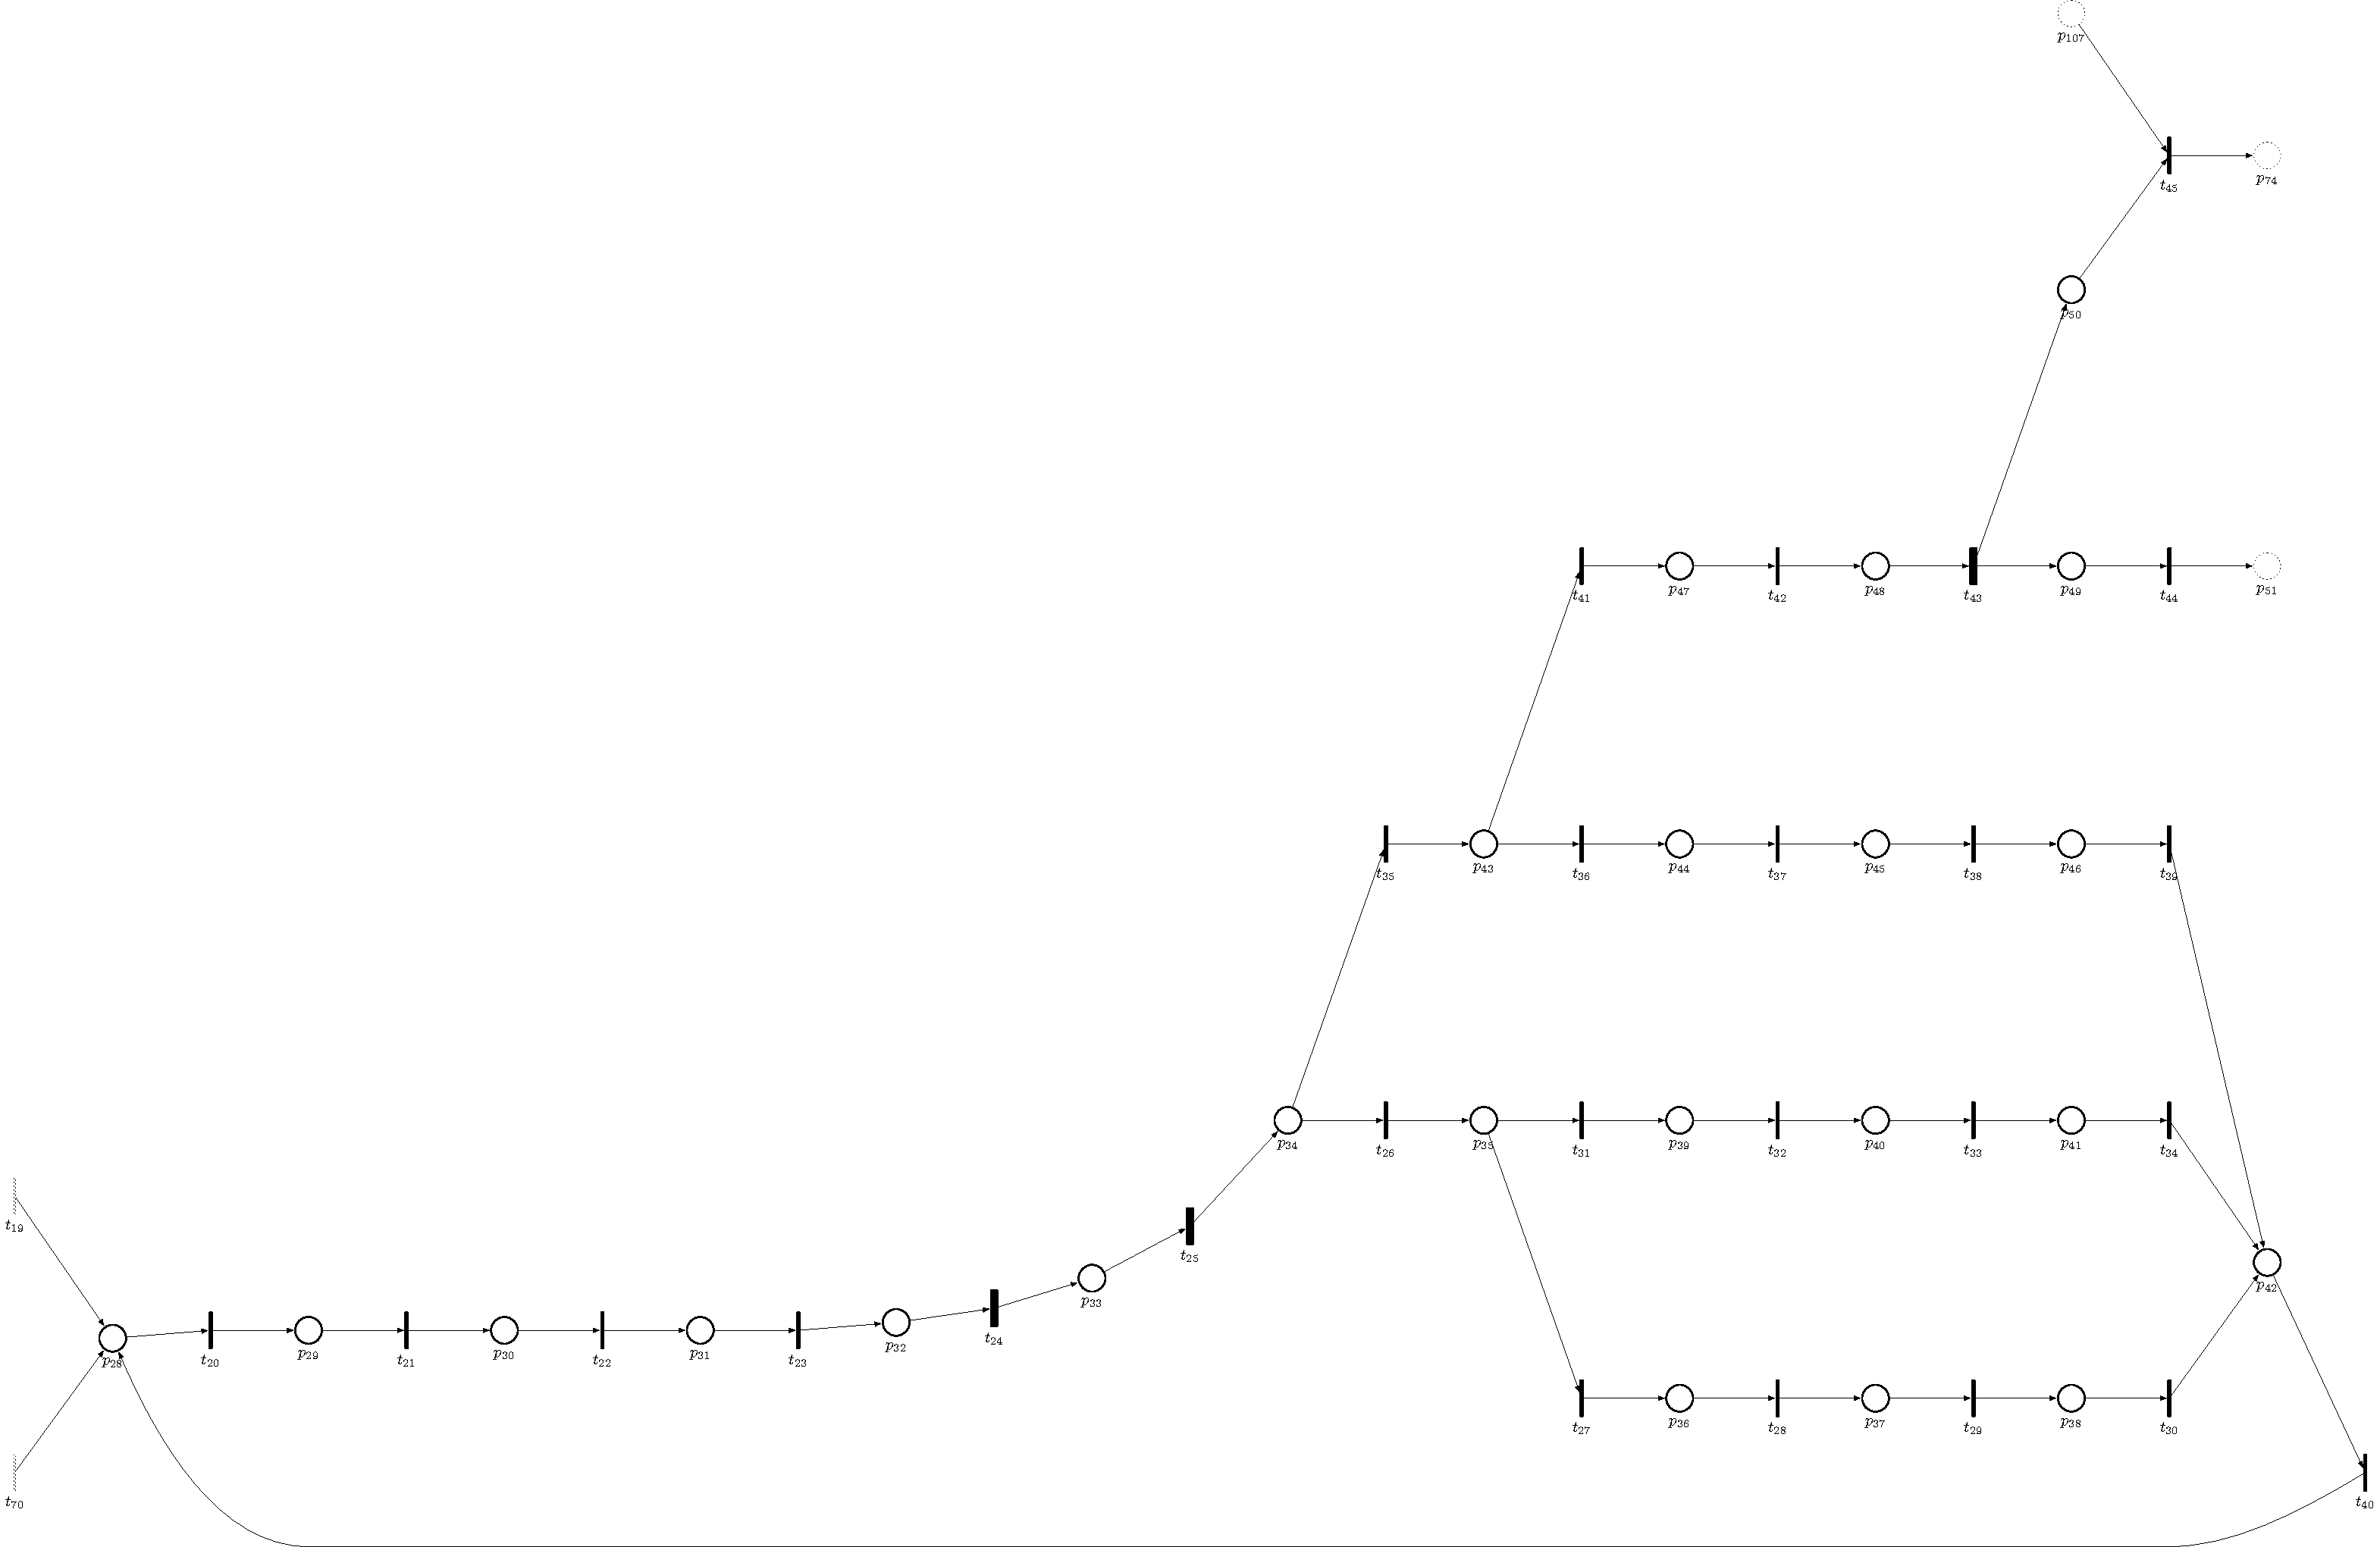
\includegraphics{../../figures/petriNets/dot/2-metalv/metalv.pdf}
%   \caption{qlksdjf}
%   \label{fig:example}
% \end{figure}


\OmegaSet

\begin{figure}[H]
  \centering
  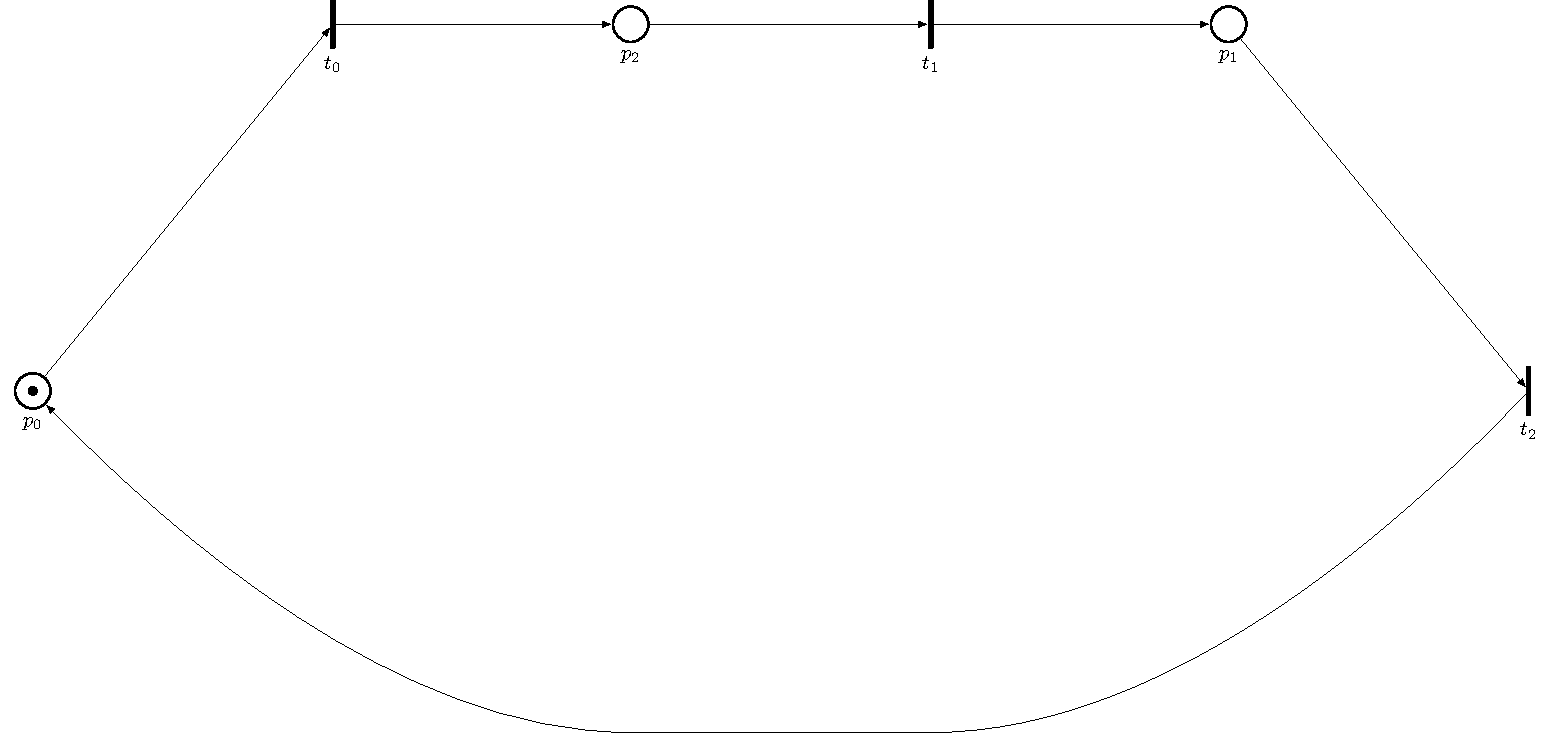
\includegraphics[width=0.4\textwidth]{../../figures/tests/teste.tikz}
  \caption{petri net example}
  \label{fig:petrinetexample}
\end{figure}


\clearpage

% \addtikzfigure{../../figures/petriNets/dot/1-initialization/initial}
% {Petri net of Initialization module.}
% {petriinitialization}
% \newpage
% \begin{table}[htbp]
\caption{Lugares do Módulo de Inicialização}
\centering
\begin{tabular}{c|c}
Places & Meaning\\
\hline
p\textsubscript{0} & System Stopped\\
p\textsubscript{1} & Retract MAG 1 Cylinder *\\
p\textsubscript{2} & MAG1's Cylinder Retracted\\
p\textsubscript{3} & Retract MAG 2 Cylinder *\\
p\textsubscript{4} & MAG2's Cylinder Recuado\\
p\textsubscript{5} & Retrair pistão de descarte D*\\
p\textsubscript{6} & Pistão de descarte D Recuado\\
p\textsubscript{7} & Retrair pistão de descarte C*\\
p\textsubscript{8} & Pistão de descarte C Recuado\\
p\textsubscript{9} & Retrair pistão de descarte E*\\
p\textsubscript{10} & Pistão de descarte E Recuado\\
p\textsubscript{11} & Ligar esteira sentido reverso\\
p\textsubscript{12} & Esteira limpa\\
p\textsubscript{13} & Resetar Variáveis\footnotemark\\
p\textsubscript{14} & Retrair atuador vertical da prensa\\
p\textsubscript{15} & Levantar porta da prensa\\
p\textsubscript{16} & Estender atuador horizontal da prensa\\
p\textsubscript{17} & Prensa pronta\\
p\textsubscript{18} & Braço retraído e armazenador de cubos retraído na horizontal\\
p\textsubscript{19} & Mover armazenador para direita\\
p\textsubscript{20} & Armazenador pronto na horizontal\\
p\textsubscript{21} & Mover armazenador para baixo\\
p\textsubscript{22} & Armazenador pronto na vertical\\
p\textsubscript{23} & Girar braço sentido antihorário\footnotemark\\
p\textsubscript{24} & Braço parado\\
p\textsubscript{25} & Girar braço sentido horário\textsuperscript{\ref{org074bf9c}} e Habilita HSC\\
p\textsubscript{26} & Braço parado frente a esteira\\
p\textsubscript{27} & Sistema Pronto\\
\end{tabular}
\end{table}\footnotetext[1]{\label{org10fa1d9}Variáveis IEC\textsubscript{COUNTER}, IEC\textsubscript{COUNTER1}, IEC\textsubscript{COUNTER2}, IEC\textsubscript{COUNTER3}, IEC\textsubscript{COUNTER4}, IEC\textsubscript{COUNTER5}.}\footnotetext[2]{\label{org074bf9c}Verificar sentido de rotação do braço.}

\begin{table}[htbp]
\caption{Transições do Módulo de Inicialização}
\centering
\begin{tabular}{ll}
Transitions & Meaning\\
t\textsubscript{0} & Botão de inicialização\\
t\textsubscript{1} & Sensor MAG 1 Retraído\\
t\textsubscript{2} & Sensor MAG 2 Retraído\\
t\textsubscript{3} & Sensor pistão de descarte D Retraído\\
t\textsubscript{4} & Sensor pistão de descarte C Retraído\\
t\textsubscript{5} & Sensor pistão de descarte E Retraído\\
t\textsubscript{6} & \\
t\textsubscript{7} & T=15s\\
t\textsubscript{8} & T=2.5s\\
t\textsubscript{9} & Sensor porta prensa aberta\\
t\textsubscript{10} & Sensor atuador horizontal da prensa estendido\\
t\textsubscript{11} & Sensor Hz armazenador de cubos e braço retraídos\\
t\textsubscript{12} & Fim de curso direito do armazenador de cubos\\
t\textsubscript{13} & Fim de curso inferior do armazenador de cubos\\
t\textsubscript{14} & T=2s\\
t\textsubscript{15} & Sensor Indutivo do braço\\
t\textsubscript{16} & T=1s\\
t\textsubscript{17} & Count\_300C.DB.Countval = \todo{-1690}\\
t\textsubscript{18} & \\
t\textsubscript{19} & Botão Começar\\
\end{tabular}
\end{table}

% \newpage
% \addtikzfigure{../../figures/petriNets/dot/2-metalv/metalv}
% {Petri net of metal cube half sorting module.}
% {petri_initialization}
% \newpage
% \begin{table}[htbp]
\caption{Lugares do Módulo 2 pt 1}
\centering
\begin{tabular}{ll}
p\textsubscript{28} & Mag1 vazio\\
p\textsubscript{29} & Mag1 com peça\\
p\textsubscript{30} & Estender Mag1 Horizontal*\\
p\textsubscript{31} & Retrair Mag1 Horizontal*\\
p\textsubscript{32} & Mag1 Horizontal retraído\\
p\textsubscript{33} & Ligar esteira sentido normal\\
p\textsubscript{34} & \\
p\textsubscript{35} & Peça de Plástico\\
p\textsubscript{36} & Ligar esteira sentido normal\\
p\textsubscript{37} & Estender Pistão de descarte D*\\
p\textsubscript{38} & Retrair Pistão de descarte D*\\
p\textsubscript{39} & Ligar esteira sentido normal\\
p\textsubscript{40} & Estender Pistão de descarte C*\\
p\textsubscript{41} & Retrair Pistão de descarte C*\\
p\textsubscript{42} & \\
p\textsubscript{43} & Peça de Metal\\
p\textsubscript{44} & Ligar esteira sentido normal\\
p\textsubscript{45} & Estender Pistão de descarte E*\\
p\textsubscript{46} & Retrair Pistão de descarte E*\\
p\textsubscript{47} & Ligar esteira sentido normal\\
p\textsubscript{48} & Ligar esteira sentido normal\\
p\textsubscript{49} & Peça Metal Pronta\\
p\textsubscript{50} & Esteira Parada\\
\end{tabular}
\end{table}


\begin{table}[htbp]
\caption{Transições do Módulo 2 pt 1}
\centering
\begin{tabular}{ll}
t\textsubscript{20} & \(\overline{\mbox{Sensor Chave de Presença de Peça Mag1}}\)\\
t\textsubscript{21} & \\
t\textsubscript{22} & Mag1 Horizontal estendido \(\uparrow\)\\
t\textsubscript{23} & Mag1 Horizontal retraído \(\uparrow\)\\
t\textsubscript{24} & T=0.5s\\
t\textsubscript{25} & Presença \(\uparrow\) T=0.5s\\
t\textsubscript{26} & \(\overline{\mbox{Sensor Metal}}\)\\
t\textsubscript{27} & Sensor Preto\\
t\textsubscript{28} & Presença Pistão de D \(\uparrow\)\\
t\textsubscript{29} & Sensor pistão de descarte D estendido\\
t\textsubscript{30} & Sensor pistão de descarte D retraído\\
t\textsubscript{31} & Sensor Branco\\
t\textsubscript{32} & Presença Pistão de C \(\uparrow\)\\
t\textsubscript{33} & Sensor pistão de descarte C estendido\\
t\textsubscript{34} & Sensor pistão de descarte C retraído\\
t\textsubscript{35} & Sensor Metal\\
t\textsubscript{36} & Sensor peça concavidade para baixo\\
t\textsubscript{37} & Presença Pistão de E \(\uparrow\)\\
t\textsubscript{38} & Sensor pistão de descarte E estendido\\
t\textsubscript{39} & Sensor pistão de descarte E retraído\\
t\textsubscript{40} & \\
t\textsubscript{41} & Sensor peça concavidade para cima\\
t\textsubscript{42} & Sensor final da esteira \(\uparrow\)\\
t\textsubscript{43} & T=0.5s\\
t\textsubscript{44} & Sensor final da esteira \(\downarrow\)\\
t\textsubscript{45} & \\
\end{tabular}
\end{table}

% \newpage
% \addtikzfigure{../../figures/petriNets/dot/3-plastic^/plastic}
% {Petri net of plastic cube half sorting module.}
% {petri_initialization}
% \newpage
% \begin{table}[htbp]
\caption{Lugares do Módulo 2 pt 2}
\centering
\begin{tabular}{ll}
P\textsubscript{51} & Mag2 vazio\\
P\textsubscript{52} & Mag2 com peça\\
P\textsubscript{53} & Estender Mag2 Horizontal*\\
p\textsubscript{54} & Retrair Mag2 Horizontal*\\
p\textsubscript{55} & Mag2 Horizontal Retraído\\
p\textsubscript{56} & Ligar esteira sentido normal\\
p\textsubscript{57} & \\
p\textsubscript{58} & Ligar esteira sentido normal\\
p\textsubscript{59} & Estender Pistão de descarte E*\\
p\textsubscript{60} & Retrair Pistão de descarte E*\\
p\textsubscript{61} & Peça de Metal\\
p\textsubscript{62} & Ligar esteira sentido normal\\
p\textsubscript{63} & Estender Pistão de descarte D*\\
p\textsubscript{64} & Retrair Pistão de descarte D*\\
p\textsubscript{65} & Peça Branca\\
p\textsubscript{66} & Ligar esteira sentido normal\\
p\textsubscript{67} & Estender Pistão de descarte C*\\
p\textsubscript{68} & Retrair Pistão de descarte C*\\
p\textsubscript{69} & \\
p\textsubscript{70} & Ligar esteira sentido normal\\
p\textsubscript{71} & Ligar esteira sentido normal\\
p\textsubscript{72} & Peça branca pronta\\
p\textsubscript{73} & Esteira parada\\
\end{tabular}
\end{table}

\begin{table}[htbp]
\caption{Transições do Módulo 2 pt 2}
\centering
\begin{tabular}{ll}
t\textsubscript{46} & \(\overline{\mbox{Sensor Chave de Presença de Peça Mag2}}\)\\
t\textsubscript{47} & \\
t\textsubscript{48} & Mag2 Horizontal estendido \(\uparrow\)\\
t\textsubscript{49} & Mag2 Horizontal retraído \(\uparrow\)\\
t\textsubscript{50} & T=0.5s\\
t\textsubscript{51} & Presença \(\uparrow\) T=0.5s\\
t\textsubscript{52} & Sensor Metal\\
t\textsubscript{53} & Presença Pistão de E \(\uparrow\)\\
t\textsubscript{54} & Sensor pistão de descarte E estendido\\
t\textsubscript{55} & Sensor pistão de descarte E retraído\\
t\textsubscript{56} & \(\overline{\mbox{Sensor Metal}}\)\\
t\textsubscript{57} & Sensor Preto\\
t\textsubscript{58} & Presença Pistão de D \(\uparrow\)\\
t\textsubscript{59} & Sensor pistão de descarte D estendido\\
t\textsubscript{60} & Sensor pistão de descarte D retraído\\
t\textsubscript{61} & Sensor Branco\\
t\textsubscript{62} & Sensor peça concavidade para cima\\
t\textsubscript{63} & Presença Pistão de C \(\uparrow\)\\
t\textsubscript{64} & Sensor pistão de descarte C estendido\\
t\textsubscript{65} & Sensor pistão de descarte C retraído\\
t\textsubscript{66} & \\
t\textsubscript{67} & Sensor peça concavidade para baixo\\
t\textsubscript{68} & Sensor final da esteira \(\uparrow\)\\
t\textsubscript{69} & T=0.5s\\
t\textsubscript{70} & Sensor final da esteira \(\downarrow\)\\
t\textsubscript{71} & \\
\end{tabular}
\end{table}

% \newpage
% \addtikzfigure{../../figures/petriNets/dot/4-armBeltToPress/armBeltToPress}
% {Petri net of manipulator taking a cube half from conveyor belt to assembly unit
%   module.}
% {petri_initialization}
% \newpage
% \begin{table}[htbp]
\caption{Lugares do Módulo Braço Esteira Prensa}
\centering
\begin{tabular}{c|c}
Places & Meaning\\
\hline
\hyperlink{partialNet:p74}{\hypertarget{partialTable:p74}{$p_{74}$}} & Estender verticalmente o braço\\
\hyperlink{partialNet:p75}{\hypertarget{partialTable:p75}{$p_{75}$}} & Estender vertical e horizontalmente o braço e Ligar o vácuo\\
\hyperlink{partialNet:p76}{\hypertarget{partialTable:p76}{$p_{76}$}} & Estender horizontalmente o braço e Ligar o vácuo\\
\hyperlink{partialNet:p77}{\hypertarget{partialTable:p77}{$p_{77}$}} & Estender vertical e horizontalmente o braço e Ligar o vácuo\\
\hyperlink{partialNet:p78}{\hypertarget{partialTable:p78}{$p_{78}$}} & Estender verticalmente o braço e Ligar o vácuo\\
\hyperlink{partialNet:p79}{\hypertarget{partialTable:p79}{$p_{79}$}} & Habilita HSC e Estender verticalmente o braço, Ligar o vácuo e Girar Braço no sentido horário\\
\hyperlink{partialNet:p80}{\hypertarget{partialTable:p80}{$p_{80}$}} & Estender vertical e horizontalmente o braço e Ligar o vácuo\\
\hyperlink{partialNet:p81}{\hypertarget{partialTable:p81}{$p_{81}$}} & Estender horizontalmente o braço e Ligar o vácuo\\
\hyperlink{partialNet:p82}{\hypertarget{partialTable:p82}{$p_{82}$}} & Estender horizontalmente o braço\\
\hyperlink{partialNet:p83}{\hypertarget{partialTable:p83}{$p_{83}$}} & Estender vertical e horizontalmente o braço\\
\hyperlink{partialNet:p84}{\hypertarget{partialTable:p84}{$p_{84}$}} & Estender verticalmente o braço\\
\hyperlink{partialNet:p85}{\hypertarget{partialTable:p85}{$p_{85}$}} & Habilita HSC e Estender verticalmente o braço e Girar Braço no sentido antihorário\\
\hyperlink{partialNet:p86}{\hypertarget{partialTable:p86}{$p_{86}$}} & Estender Verticalmente o braço e IEC\(_{\text{COUNTER}}\):=IEC\(_{\text{COUNTER}}\)+1\\
\end{tabular}
\end{table}

\begin{table}[htbp]
\caption{Transições do Módulo Braço Esteira Prensa}
\centering
\begin{tabular}{c|c}
Transitions & Meaning\\
\hline
\hyperlink{partialNet:t72}{\hypertarget{partialTable:t72}{$t_{72}$}} & Sensor vertical braço estendido\\
\hyperlink{partialNet:tt73}{\hypertarget{partialTable:tt73}{$t_{73}$}} & T=1.5s\\
\hyperlink{partialNet:tt74}{\hypertarget{partialTable:tt74}{$t_{74}$}} & T=1.5s e Sensor vertical braço retraído\\
\hyperlink{partialNet:tt75}{\hypertarget{partialTable:tt75}{$t_{75}$}} & T=1.5s e Sensor vertical braço estendido\\
\hyperlink{partialNet:tt76}{\hypertarget{partialTable:tt76}{$t_{76}$}} & T=1.5s e Sensor vertical braço estendido\\
\hyperlink{partialNet:t77}{\hypertarget{partialTable:t77}{$t_{77}$}} & Count\_300C.DB.CountVal = \todo{-3330}\\
\hyperlink{partialNet:tt78}{\hypertarget{partialTable:tt78}{$t_{78}$}} & T=1.5s e Sensor vertical braço estendido\\
\hyperlink{partialNet:tt79}{\hypertarget{partialTable:tt79}{$t_{79}$}} & T=1.5s e Sensor vertical braço retraído\\
\hyperlink{partialNet:tt80}{\hypertarget{partialTable:tt80}{$t_{80}$}} & T=1.5s\\
\hyperlink{partialNet:tt81}{\hypertarget{partialTable:tt81}{$t_{81}$}} & T=1.5s e Sensor vertical braço estendido\\
\hyperlink{partialNet:t82}{\hypertarget{partialTable:t82}{$t_{82}$}} & IEC\(_{\text{COUNTER0.DB}}\)=1 e Sensor Hz prensa estendido e porta prensa aberta\\
\hyperlink{partialNet:tt83}{\hypertarget{partialTable:tt83}{$t_{83}$}} & T=1.5s e IEC\(_{\text{COUNTER0.DB}}\)=0 e Sensor vertical braço estendido\\
\hyperlink{partialNet:t84}{\hypertarget{partialTable:t84}{$t_{84}$}} & Count\_300C.DB.CountVal = \todo{-1690}\\
\hyperlink{partialNet:t85}{\hypertarget{partialTable:t85}{$t_{85}$}} & \\
\end{tabular}
\end{table}

% \clearpage
% \pagebreak
% \addtikzfigure{../../figures/petriNets/dot/5-press/press}
% {Petri net of assembly unit module.}
% {petri_initialization}
% \newpage
% \begin{table}[htbp]
\caption{Lugares do Módulo prensa cubo}
\centering
\begin{tabular}{c|c}
Places & Meaning\\
\hline
\hyperlink{partialNet:p87}{\hypertarget{partialTable:p87}{$p_{87}$}} & Retrair atuador horizontal prensa*\\
\hyperlink{partialNet:p88}{\hypertarget{partialTable:p88}{$p_{88}$}} & Fechar Porta prensa*\\
\hyperlink{partialNet:p89}{\hypertarget{partialTable:p89}{$p_{89}$}} & Estender atuador vertical prensa*\\
\hyperlink{partialNet:p90}{\hypertarget{partialTable:p90}{$p_{90}$}} & Retrair atuador vertical prensa*\\
\hyperlink{partialNet:p91}{\hypertarget{partialTable:p91}{$p_{91}$}} & Abrir Porta prensa*\\
\hyperlink{partialNet:p92}{\hypertarget{partialTable:p92}{$p_{92}$}} & Estender atuador horizontal prensa*\\
\hyperlink{partialNet:p93}{\hypertarget{partialTable:p93}{$p_{93}$}} & Cubo pronto\\
\hyperlink{partialNet:p94}{\hypertarget{partialTable:p94}{$p_{94}$}} & Estender horizontalmente o braço e Ligar Vácuo\\
\hyperlink{partialNet:p95}{\hypertarget{partialTable:p95}{$p_{95}$}} & Estender verticalmente o braço\\
 & \\
\end{tabular}
\end{table}

\begin{center}
\begin{tabular}{c|c}
Transitions & Meaning\\
\hline
\hyperlink{partialNet:tt86}{\hypertarget{partialTable:tt86}{$t_{86}$}} & T=1s e Sensosr horizontal prensa retraído\\
\hyperlink{partialNet:tt87}{\hypertarget{partialTable:tt87}{$t_{87}$}} & T=1s e Sensor porta fechada\\
\hyperlink{partialNet:tt88}{\hypertarget{partialTable:tt88}{$t_{88}$}} & T=1s\\
\hyperlink{partialNet:tt89}{\hypertarget{partialTable:tt89}{$t_{89}$}} & T=1s\\
\hyperlink{partialNet:tt90}{\hypertarget{partialTable:tt90}{$t_{90}$}} & T=1s e sensor porta aberta\\
\hyperlink{partialNet:tt91}{\hypertarget{partialTable:tt91}{$t_{91}$}} & T=1s e sensor horizontal prensa estendido\\
\hyperlink{partialNet:t92}{\hypertarget{partialTable:t92}{$t_{92}$}} & \\
\hyperlink{partialNet:tt93}{\hypertarget{partialTable:tt93}{$t_{93}$}} & T=1.5s e Sensor horizontal do braço estendido\\
\end{tabular}
\end{center}

% \newpage
% \addtikzfigure{../../figures/petriNets/dot/6-armPressToStorage/armPressToStorage}
% {Petri net of manipulator taking cube from assembly unit to storage module.}
% {petri_initialization}
% \newpage
% \begin{table}[htbp]
\caption{Lugares do Módulo braço prensa armazenador}
\centering
\begin{tabular}{ll}
Places & Meaning\\
\hline
\hyperlink{partialNet:p96}{\hypertarget{partialTable:p96}{$p_{96}$}} & Estender horizontalmente o braço e Ligar Vácuo\\
\hyperlink{partialNet:p97}{\hypertarget{partialTable:p97}{$p_{97}$}} & Estender vertical e horizontalmente o braço e Ligar Vácuo\\
\hyperlink{partialNet:p98}{\hypertarget{partialTable:p98}{$p_{98}$}} & Resetar IEC\(_{\text{COUNTER0}}\)*, estender verticalmente o braço e Ligar Vácuo\\
\hyperlink{partialNet:p99}{\hypertarget{partialTable:p99}{$p_{99}$}} & Habilita HSC e Estender verticalmente o braço, Ligar Vácuo e Girar o Braço no sentido horário\\
\hyperlink{partialNet:p100}{\hypertarget{partialTable:p100}{$p_{100}$}} & Estender vertical e horizontalmente o braço e Ligar Vácuo\\
\hyperlink{partialNet:p101}{\hypertarget{partialTable:p101}{$p_{101}$}} & Estender horizontalmente o braço e Ligar Vácuo\\
\hyperlink{partialNet:p102}{\hypertarget{partialTable:p102}{$p_{102}$}} & Estender horizontalmente o braço\\
\hyperlink{partialNet:p103}{\hypertarget{partialTable:p103}{$p_{103}$}} & Estender vertical e horizontalmente o braço\\
\hyperlink{partialNet:p104}{\hypertarget{partialTable:p104}{$p_{104}$}} & Girar o braço no sentido antihorário\\
\hyperlink{partialNet:p105}{\hypertarget{partialTable:p105}{$p_{105}$}} & Braço parado\\
\hyperlink{partialNet:p106}{\hypertarget{partialTable:p106}{$p_{106}$}} & Habilita HSC e Girar o braço no sentido horário\\
\hyperlink{partialNet:p107}{\hypertarget{partialTable:p107}{$p_{107}$}} & Braço na esteira\\
\end{tabular}
\end{table}

\begin{table}[htbp]
\caption{Transições do Módulo braço prensa armazenador}
\centering
\begin{tabular}{ll}
Transitions & Meaning\\
\hline
\hyperlink{partialNet:tt94}{\hypertarget{partialTable:tt94}{$t_{94}$}} & T=1.5s e Sensor vertical braço retraído\\
\hyperlink{partialNet:t95}{\hypertarget{partialTable:t95}{$t_{95}$}} & Sensor vertical braço estendido, Fim de curso inferior e direito armazenador\\
\hyperlink{partialNet:t96}{\hypertarget{partialTable:t96}{$t_{96}$}} & \\
\hyperlink{partialNet:t97}{\hypertarget{partialTable:t97}{$t_{97}$}} & Count\_300C.DB.CountVal = \todo{-4920}\\
\hyperlink{partialNet:tt98}{\hypertarget{partialTable:tt98}{$t_{98}$}} & T=2s\\
\hyperlink{partialNet:tt99}{\hypertarget{partialTable:tt99}{$t_{99}$}} & T=2s\\
\hyperlink{partialNet:t100}{\hypertarget{partialTable:t100}{$t_{100}$}} & Sensor vertical braço retraído\\
\hyperlink{partialNet:t101}{\hypertarget{partialTable:t101}{$t_{101}$}} & Sensor vertical braço estendido, Fim de curso inferior e direito armazenador\\
\hyperlink{partialNet:t102}{\hypertarget{partialTable:t102}{$t_{102}$}} & Sensor indutivo do braço\\
\hyperlink{partialNet:tt103}{\hypertarget{partialTable:tt103}{$t_{103}$}} & T=1s\\
\hyperlink{partialNet:t104}{\hypertarget{partialTable:t104}{$t_{104}$}} & Count\_300C.DB.CountVal = \todo{-1690}\\
\end{tabular}
\end{table}

% \newpage
% \addtikzfigure{../../figures/petriNets/dot/7-storageY/storageY}
% {Petri net of storage unit positioning module (y axis).}
% {petri_initialization}
% \newpage
% \begin{table}[htbp]
\caption{Storage Unit (Y axis) Module Places.}
\centering
\begin{tabular}{cc}
Places & Meaning\\
\hline
\hyperlink{partialNet:p108}{\hypertarget{partialTable:p108}{$p_{108}$}} & Cube on Storage Unit\\
\hyperlink{partialNet:p109}{\hypertarget{partialTable:p109}{$p_{109}$}} & Move Storage Unit to the Right\\
\hyperlink{partialNet:p110}{\hypertarget{partialTable:p110}{$p_{110}$}} & \\
\hyperlink{partialNet:p111}{\hypertarget{partialTable:p111}{$p_{111}$}} & Move Storage Unit Upwards\\
\hyperlink{partialNet:p112}{\hypertarget{partialTable:p112}{$p_{112}$}} & Move Storage Unit Upwards\\
\hyperlink{partialNet:p113}{\hypertarget{partialTable:p113}{$p_{113}$}} & Move Storage Unit Upwards\\
\hyperlink{partialNet:p114}{\hypertarget{partialTable:p114}{$p_{114}$}} & Move Storage Unit Upwards\\
\hyperlink{partialNet:p115}{\hypertarget{partialTable:p115}{$p_{115}$}} & COUNTER3:=COUNTER3+1\\
\hyperlink{partialNet:p116}{\hypertarget{partialTable:p116}{$p_{116}$}} & RESET COUNTER3*\\
\hyperlink{partialNet:p117}{\hypertarget{partialTable:p117}{$p_{117}$}} & \\
\end{tabular}
\end{table}


\begin{table}[htbp]
\caption{Storage Unit (Y axis) Module Transitions.}
\centering
\begin{tabular}{cc}
Transitions & Meaning\\
\hline
\hyperlink{partialNet:tt105}{\hypertarget{partialTable:tt105}{$t_{105}$}} & T=2s\\
\hyperlink{partialNet:tt106}{\hypertarget{partialTable:tt106}{$t_{106}$}} & T=2s\\
\hyperlink{partialNet:t107}{\hypertarget{partialTable:t107}{$t_{107}$}} & COUNTER2=0\\
\hyperlink{partialNet:t108}{\hypertarget{partialTable:t108}{$t_{108}$}} & COUNTER3=4\\
\hyperlink{partialNet:t109}{\hypertarget{partialTable:t109}{$t_{109}$}} & Vertical Encoder\\
\hyperlink{partialNet:t110}{\hypertarget{partialTable:t110}{$t_{110}$}} & COUNTER2=1\\
\hyperlink{partialNet:t111}{\hypertarget{partialTable:t111}{$t_{111}$}} & COUNTER3=3\\
\hyperlink{partialNet:t112}{\hypertarget{partialTable:t112}{$t_{112}$}} & Vertical Encoder\\
\hyperlink{partialNet:t113}{\hypertarget{partialTable:t113}{$t_{113}$}} & COUNTER2=2\\
\hyperlink{partialNet:t114}{\hypertarget{partialTable:t114}{$t_{114}$}} & COUNTER3=2\\
\hyperlink{partialNet:t115}{\hypertarget{partialTable:t115}{$t_{115}$}} & Vertical Encoder\\
\hyperlink{partialNet:t116}{\hypertarget{partialTable:t116}{$t_{116}$}} & COUNTER2=3\\
\hyperlink{partialNet:t117}{\hypertarget{partialTable:t117}{$t_{117}$}} & COUNTER3=1\\
\hyperlink{partialNet:t118}{\hypertarget{partialTable:t118}{$t_{118}$}} & Vertical Encoder\\
\hyperlink{partialNet:t119}{\hypertarget{partialTable:t119}{$t_{119}$}} & \\
\hyperlink{partialNet:t120}{\hypertarget{partialTable:t120}{$t_{120}$}} & \\
\end{tabular}
\end{table}

% \newpage
% \addtikzfigure{../../figures/petriNets/dot/8-storageX/storageX}
% {Petri net of storage unit positioning module (x axis).}
% {petri_initialization}
% \newpage
% \begin{table}[htbp]
\caption{Lugares do Módulo armazenador (x)}
\centering
\begin{tabular}{ll}
p\textsubscript{120} & COUNTER1:=COUNTER1+1 e COUNTER4:=COUNTER4+1\\
p\textsubscript{121} & COUNTER5:=COUNTER5+1 e mover armazenador para a esquerda\\
p\textsubscript{122} & Reset COUNTER5*\\
p\textsubscript{123} & COUNTER5:=COUNTER5+1 e mover armazenador para a esquerda\\
p\textsubscript{124} & Reset COUNTER5*\\
p\textsubscript{125} & COUNTER5:=COUNTER5+1 e mover armazenador para a esquerda\\
p\textsubscript{126} & Reset COUNTER5*\\
p\textsubscript{127} & COUNTER5:=COUNTER5+1 e mover armazenador para a esquerda\\
p\textsubscript{128} & Reset COUNTER5*\\
p\textsubscript{129} & COUNTER5:=COUNTER5+1 e mover armazenador para a esquerda\\
p\textsubscript{130} & Reset COUNTER5*\\
p\textsubscript{131} & COUNTER5:=COUNTER5+1 e mover armazenador para a esquerda\\
p\textsubscript{132} & Reset COUNTER5*\\
p\textsubscript{133} & COUNTER5:=COUNTER5+1 e mover armazenador para a esquerda\\
p\textsubscript{134} & Reset COUNTER5* Reset COUNTER4* , COUNTER2:=COUNTER2+1\\
p\textsubscript{135} & \\
\end{tabular}
\end{table}

\begin{table}[htbp]
\caption{Transições Módulo armazenador (x)}
\centering
\begin{tabular}{ll}
t\textsubscript{119} & COUNTER4=0\\
t\textsubscript{120} & COUNTER5=1\\
t\textsubscript{121} & \\
t\textsubscript{122} & COUNTER4=1\\
t\textsubscript{123} & COUNTER5=2\\
t\textsubscript{124} & \\
t\textsubscript{125} & COUNTER4=2\\
t\textsubscript{126} & COUNTER5=3\\
t\textsubscript{127} & \\
t\textsubscript{128} & COUNTER4=3\\
t\textsubscript{129} & COUNTER5=4\\
t\textsubscript{130} & \\
t\textsubscript{131} & COUNTER4=4\\
t\textsubscript{132} & COUNTER5=5\\
t\textsubscript{133} & \\
t\textsubscript{134} & COUNTER4=5\\
t\textsubscript{135} & COUNTER5=8\\
t\textsubscript{136} & \\
t\textsubscript{137} & COUNTER4=6\\
t\textsubscript{138} & COUNTER5=9\\
t\textsubscript{139} & \\
\end{tabular}
\end{table}

% \newpage
% \addtikzfigure{../../figures/petriNets/dot/9-storePiece/storePiece}
% {Petri net of cube storage module.}
% {petri_initialization}
% \newpage

\begin{table}[htbp]
\caption{Places from the cube storage module.}
\centering
\begin{tabular}{ll}
p\(_{\text{136}}\) & Estender horizontalmente armazenador\\
p\(_{\text{137}}\) & Estender horizontalmente armazenador e mover armazenador para baixo\\
p\(_{\text{138}}\) & Estender horizontalmente armazenador\\
p\(_{\text{139}}\) & Peça armazenada\\
p\(_{\text{140}}\) & Mover armazenador para a direita\\
p\(_{\text{141}}\) & Armazenador pronto na horizontal\\
p\(_{\text{142}}\) & Mover armazenador para baixo\\
p\(_{\text{143}}\) & Armazenador pronto na vertical\\
p\(_{\text{144}}\) & \\
p\(_{\text{145}}\) & Armazenador pronto\\
\end{tabular}
\end{table}

\begin{table}[htbp]
\caption{Transitions from the cube storage module.}
\centering
\begin{tabular}{ll}
t\(_{\text{140}}\) & T=2s\\
t\(_{\text{141}}\) & T=3s\\
t\(_{\text{142}}\) & T=0.25s\\
t\(_{\text{143}}\) & T=3s\\
t\(_{\text{144}}\) & T=7s\\
t\(_{\text{145}}\) & Fim de curso direito do armazenador\\
t\(_{\text{146}}\) & Fim de curso inferior do armazenador\\
t\(_{\text{147}}\) & \\
t\(_{\text{148}}\) & COUNTER1<28\\
t\(_{\text{149}}\) & COUNTER1=28\\
\end{tabular}
\end{table}


\begin{longtable}{m{5cm}m{5cm}}
\caption{Complete Places.}
\\
Places & Meaning\\
\hline
\endfirsthead
\multicolumn{2}{l}{Continued from previous page} \\
\hline

Places & Meaning \\

\hline
\endhead
\hline\multicolumn{2}{r}{Continued on next page} \\
\endfoot
\endlastfoot
\hline
\hyperlink{completeNet:p0}{\hypertarget{completeTable:p0m1}{$p_{0}$}} & System Stopped\\
\hyperlink{completeNet:p1}{\hypertarget{completeTable:p1}{$p_{1}$}}, \hyperlink{completeNet:p31}{\hypertarget{completeTable:p31}{$p_{31}$}} & Retract MAG1's Cylinder *\\
\hyperlink{completeNet:p2}{\hypertarget{completeTable:p2}{$p_{2}$}}, \hyperlink{completeNet:p32}{\hypertarget{completeTable:p32}{$p_{32}$}} & MAG1's Cylinder Retracted\\
\hyperlink{completeNet:p3}{\hypertarget{completeTable:p3}{$p_{3}$}}, \hyperlink{completeNet:p54}{\hypertarget{completeTable:p54}{$p_{54}$}} & Retract MAG2's Cylinder *\\
\hyperlink{completeNet:p4}{\hypertarget{completeTable:p4}{$p_{4}$}}, \hyperlink{completeNet:p55}{\hypertarget{completeTable:p55}{$p_{55}$}} & MAG2's Cylinder Retracted\\
\hyperlink{completeNet:p5}{\hypertarget{completeTable:p5}{$p_{5}$}}, \hyperlink{completeNet:p38}{\hypertarget{completeTable:p38}{$p_{38}$}}, \hyperlink{completeNet:p64}{\hypertarget{completeTable:p64}{$p_{64}$}} & Retract Right Discharge Cylinder *\\
\hyperlink{completeNet:p6}{\hypertarget{completeTable:p6}{$p_{6}$}} & Right Discharge Cylinder Retracted\\
\hyperlink{completeNet:p7}{\hypertarget{completeTable:p7}{$p_{7}$}} & Retract Center Discharge Cylinder\\
\hyperlink{completeNet:p8}{\hypertarget{completeTable:p8}{$p_{8}$}} & Center Discharge Cylinder Retracted\\
\hyperlink{completeNet:p9}{\hypertarget{completeTable:p9}{$p_{9}$}}, \hyperlink{completeNet:p46}{\hypertarget{completeTable:p46}{$p_{46}$}}, \hyperlink{completeNet:p60}{\hypertarget{completeTable:p60}{$p_{60}$}} & Retract Left Discharge Cylinder *\\
\hyperlink{completeNet:p10}{\hypertarget{completeTable:p10}{$p_{10}$}} & Left Discharge Cylinder Retracted\\
\hyperlink{completeNet:p11}{\hypertarget{completeTable:p11}{$p_{11}$}} & Turn Conveyor Belt On (Reverse)\\
\hyperlink{completeNet:p12}{\hypertarget{completeTable:p12}{$p_{12}$}} & No Pieces On Conveyor Belt\\
\hyperlink{completeNet:p13}{\hypertarget{completeTable:p13}{$p_{13}$}} & Reset Variables\\
\hyperlink{completeNet:p14}{\hypertarget{completeTable:p14}{$p_{14}$}} & Raise Press\\
\hyperlink{completeNet:p15}{\hypertarget{completeTable:p15}{$p_{15}$}} & Open Safety Door\\
\hyperlink{completeNet:p16}{\hypertarget{completeTable:p16}{$p_{16}$}} & Extend Assembly Unit Holder\\
\hyperlink{completeNet:p17}{\hypertarget{completeTable:p17}{$p_{17}$}} & Assembly Unit Ready\\
\hyperlink{completeNet:p18}{\hypertarget{completeTable:p18}{$p_{18}$}} & Arm Lowered and Retracted, and Storage Unit Retracted\\
\hyperlink{completeNet:p19}{\hypertarget{completeTable:p19}{$p_{19}$}}, \hyperlink{completeNet:p109}{\hypertarget{completeTable:p109}{$p_{109}$}}, \hyperlink{completeNet:p134}{\hypertarget{completeTable:p134}{$p_{134}$}} & Move Storage Unit to the Right\\
\hyperlink{completeNet:p20}{\hypertarget{completeTable:p20}{$p_{20}$}} & Storage Unit ready ( horizontal )\\
\hyperlink{completeNet:p21}{\hypertarget{completeTable:p21}{$p_{21}$}} & Move Storage Device Downwards\\
\hyperlink{completeNet:p22}{\hypertarget{completeTable:p22}{$p_{22}$}} & Storage Unit ready ( vertical )\\
\hyperlink{completeNet:p23}{\hypertarget{completeTable:p23}{$p_{23}$}} & Rotate Arm CCW\\
\hyperlink{completeNet:p24}{\hypertarget{completeTable:p24}{$p_{24}$}} & Arm Stopped\\
\hyperlink{completeNet:p25}{\hypertarget{completeTable:p25}{$p_{25}$}} & Rotate Arm CW e Turn HSC ON\\
\hyperlink{completeNet:p26}{\hypertarget{completeTable:p26}{$p_{26}$}}, \hyperlink{completeNet:p107}{\hypertarget{completeTable:p107}{$p_{107}$}} & Arm Stopped ( facing conveyor belt )\\
\hyperlink{completeNet:p27}{\hypertarget{completeTable:p27}{$p_{27}$}} & System Ready\\
\hyperlink{completeNet:p28}{\hypertarget{completeTable:p28}{$p_{28}$}} & MAG1 Empty\\
\hyperlink{completeNet:p29}{\hypertarget{completeTable:p29}{$p_{29}$}} & MAG1 Not Empty\\
\hyperlink{completeNet:p30}{\hypertarget{completeTable:p30}{$p_{30}$}} & Extend MAG1's Cylinder *\\
\hyperlink{completeNet:p33}{\hypertarget{completeTable:p33}{$p_{33}$}}, \hyperlink{completeNet:p36}{\hypertarget{completeTable:p36}{$p_{36}$}}, \hyperlink{completeNet:p39}{\hypertarget{completeTable:p39}{$p_{39}$}}, \hyperlink{completeNet:p44}{\hypertarget{completeTable:p44}{$p_{44}$}}, \hyperlink{completeNet:p47}{\hypertarget{completeTable:p47}{$p_{47}$}}, \hyperlink{completeNet:p48}{\hypertarget{completeTable:p48}{$p_{48}$}}, \hyperlink{completeNet:p56}{\hypertarget{completeTable:p56}{$p_{56}$}}, \hyperlink{completeNet:p58}{\hypertarget{completeTable:p58}{$p_{58}$}}, \hyperlink{completeNet:p62}{\hypertarget{completeTable:p62}{$p_{62}$}}, \hyperlink{completeNet:p66}{\hypertarget{completeTable:p66}{$p_{66}$}}, \hyperlink{completeNet:p70}{\hypertarget{completeTable:p70}{$p_{70}$}}, \hyperlink{completeNet:p71}{\hypertarget{completeTable:p71}{$p_{71}$}} & Turn Conveyor Belt On\\
\hyperlink{completeNet:p34}{\hypertarget{completeTable:p34}{$p_{34}$}}, \hyperlink{completeNet:p42}{\hypertarget{completeTable:p42}{$p_{42}$}}, \hyperlink{completeNet:p57}{\hypertarget{completeTable:p57}{$p_{57}$}}, \hyperlink{completeNet:p69}{\hypertarget{completeTable:p69}{$p_{69}$}}, \hyperlink{completeNet:p110}{\hypertarget{completeTable:p110}{$p_{110}$}}, \hyperlink{completeNet:p117}{\hypertarget{completeTable:p117}{$p_{117}$}}, \hyperlink{completeNet:p129}{\hypertarget{completeTable:p129}{$p_{129}$}}, \hyperlink{completeNet:p138}{\hypertarget{completeTable:p138}{$p_{138}$}} & \\
\hyperlink{completeNet:p35}{\hypertarget{completeTable:p35}{$p_{35}$}} & Plastic Half-cube\\
\hyperlink{completeNet:p37}{\hypertarget{completeTable:p37}{$p_{37}$}}, \hyperlink{completeNet:p63}{\hypertarget{completeTable:p63}{$p_{63}$}} & Extend Right Discharge Cylinder *\\
\hyperlink{completeNet:p40}{\hypertarget{completeTable:p40}{$p_{40}$}}, \hyperlink{completeNet:p67}{\hypertarget{completeTable:p67}{$p_{67}$}} & Extend Center Discharge Cylinder *\\
\hyperlink{completeNet:p41}{\hypertarget{completeTable:p41}{$p_{41}$}}, \hyperlink{completeNet:p68}{\hypertarget{completeTable:p68}{$p_{68}$}} & Retract Center Discharge Cylinder *\\
\hyperlink{completeNet:p43}{\hypertarget{completeTable:p43}{$p_{43}$}}, \hyperlink{completeNet:p61}{\hypertarget{completeTable:p61}{$p_{61}$}} & Metal Half-cube\\
\hyperlink{completeNet:p45}{\hypertarget{completeTable:p45}{$p_{45}$}}, \hyperlink{completeNet:p59}{\hypertarget{completeTable:p59}{$p_{59}$}} & Extend Left Discharge Cylinder *\\
\hyperlink{completeNet:p49}{\hypertarget{completeTable:p49}{$p_{49}$}} & Metal Half-cube Ready\\
\hyperlink{completeNet:p50}{\hypertarget{completeTable:p50}{$p_{50}$}}, \hyperlink{completeNet:p73}{\hypertarget{completeTable:p73}{$p_{73}$}} & Conveyor Belt Stopped\\
\hyperlink{completeNet:p51}{\hypertarget{completeTable:p51}{$p_{51}$}} & MAG2 Empty\\
\hyperlink{completeNet:p52}{\hypertarget{completeTable:p52}{$p_{52}$}} & MAG2 Not Empty\\
\hyperlink{completeNet:p53}{\hypertarget{completeTable:p53}{$p_{53}$}} & Extend MAG2's Cylinder *\\
\hyperlink{completeNet:p65}{\hypertarget{completeTable:p65}{$p_{65}$}} & White Half-Cube\\
\hyperlink{completeNet:p72}{\hypertarget{completeTable:p72}{$p_{72}$}} & Plastic Half-cube Ready\\
\hyperlink{completeNet:p74}{\hypertarget{completeTable:p74}{$p_{74}$}}, \hyperlink{completeNet:p84}{\hypertarget{completeTable:p84}{$p_{84}$}}, \hyperlink{completeNet:p95}{\hypertarget{completeTable:p95}{$p_{95}$}} & Raise Arm\\
\hyperlink{completeNet:p75}{\hypertarget{completeTable:p75}{$p_{75}$}} & Raise and Extend Arm, and Turn Vacuum On\\
\hyperlink{completeNet:p76}{\hypertarget{completeTable:p76}{$p_{76}$}}, \hyperlink{completeNet:p81}{\hypertarget{completeTable:p81}{$p_{81}$}}, \hyperlink{completeNet:p94}{\hypertarget{completeTable:p94}{$p_{94}$}}, \hyperlink{completeNet:p101}{\hypertarget{completeTable:p101}{$p_{101}$}} & Extend Arm and Turn Vacuum On\\
\hyperlink{completeNet:p77}{\hypertarget{completeTable:p77}{$p_{77}$}}, \hyperlink{completeNet:p80}{\hypertarget{completeTable:p80}{$p_{80}$}}, \hyperlink{completeNet:p97}{\hypertarget{completeTable:p97}{$p_{97}$}}, \hyperlink{completeNet:p100}{\hypertarget{completeTable:p100}{$p_{100}$}} & Raise and Extend Arm and Turn Vacuum On\\
\hyperlink{completeNet:p78}{\hypertarget{completeTable:p78}{$p_{78}$}} & Raise Arm and Turn Vacuum On\\
\hyperlink{completeNet:p79}{\hypertarget{completeTable:p79}{$p_{79}$}} & Turn HSC On e Raise Arm, Turn Vacuum On and Rotate Arm CW\\
\hyperlink{completeNet:p82}{\hypertarget{completeTable:p82}{$p_{82}$}}, \hyperlink{completeNet:p102}{\hypertarget{completeTable:p102}{$p_{102}$}} & Extend Arm\\
\hyperlink{completeNet:p83}{\hypertarget{completeTable:p83}{$p_{83}$}}, \hyperlink{completeNet:p103}{\hypertarget{completeTable:p103}{$p_{103}$}} & Raise and Extend Arm\\
\hyperlink{completeNet:p85}{\hypertarget{completeTable:p85}{$p_{85}$}} & Turn HSC On, Raise Arm and Rotate Arm CCW\\
\hyperlink{completeNet:p86}{\hypertarget{completeTable:p86}{$p_{86}$}} & Raise Arm and HALFPIECECOUNTER:=HALFPIECECOUNTER+1\\
\hyperlink{completeNet:p87}{\hypertarget{completeTable:p87}{$p_{87}$}} & Retract Assembly Unit Holder *\\
\hyperlink{completeNet:p88}{\hypertarget{completeTable:p88}{$p_{88}$}} & Close Safety Door *\\
\hyperlink{completeNet:p89}{\hypertarget{completeTable:p89}{$p_{89}$}} & Lower Press *\\
\hyperlink{completeNet:p90}{\hypertarget{completeTable:p90}{$p_{90}$}} & Raise Press *\\
\hyperlink{completeNet:p91}{\hypertarget{completeTable:p91}{$p_{91}$}} & Open Safety Door *\\
\hyperlink{completeNet:p92}{\hypertarget{completeTable:p92}{$p_{92}$}} & Extend Assembly Unit Holder *\\
\hyperlink{completeNet:p93}{\hypertarget{completeTable:p93}{$p_{93}$}} & Cube Ready\\
\hyperlink{completeNet:p96}{\hypertarget{completeTable:p96}{$p_{96}$}} & Extend Arm e Turn Vacuum On\\
\hyperlink{completeNet:p98}{\hypertarget{completeTable:p98}{$p_{98}$}} & Reset HALFPIECECOUNTER*, Raise Arm and Turn Vacuum On\\
\hyperlink{completeNet:p99}{\hypertarget{completeTable:p99}{$p_{99}$}} & Turn HSC On, Raise Arm, Turn Vacuum On, Rotate Arm CW\\
\hyperlink{completeNet:p104}{\hypertarget{completeTable:p104}{$p_{104}$}} & Turn Arm CCW\\
\hyperlink{completeNet:p105}{\hypertarget{completeTable:p105}{$p_{105}$}} & Arm Stoppen\\
\hyperlink{completeNet:p106}{\hypertarget{completeTable:p106}{$p_{106}$}} & Turn HSC On, Turn Arm CW\\
\hyperlink{completeNet:p108}{\hypertarget{completeTable:p108}{$p_{108}$}} & Cube on Storage Unit\\
\hyperlink{completeNet:p111}{\hypertarget{completeTable:p111}{$p_{111}$}}, \hyperlink{completeNet:p112}{\hypertarget{completeTable:p112}{$p_{112}$}}, \hyperlink{completeNet:p113}{\hypertarget{completeTable:p113}{$p_{113}$}}, \hyperlink{completeNet:p114}{\hypertarget{completeTable:p114}{$p_{114}$}} & Move Storage Unit Upwards\\
\hyperlink{completeNet:p115}{\hypertarget{completeTable:p115}{$p_{115}$}} & COUNTER3:=COUNTER3+1\\
\hyperlink{completeNet:p116}{\hypertarget{completeTable:p116}{$p_{116}$}} & RESET COUNTER3*\\
\hyperlink{completeNet:p118}{\hypertarget{completeTable:p118}{$p_{118}$}} & COUNTER1:=COUNTER1+1 e COUNTER4:=COUNTER4+1\\
\hyperlink{completeNet:p119}{\hypertarget{completeTable:p119}{$p_{119}$}}, \hyperlink{completeNet:p120}{\hypertarget{completeTable:p120}{$p_{120}$}}, \hyperlink{completeNet:p121}{\hypertarget{completeTable:p121}{$p_{121}$}}, \hyperlink{completeNet:p122}{\hypertarget{completeTable:p122}{$p_{122}$}}, \hyperlink{completeNet:p123}{\hypertarget{completeTable:p123}{$p_{123}$}}, \hyperlink{completeNet:p124}{\hypertarget{completeTable:p124}{$p_{124}$}}, \hyperlink{completeNet:p125}{\hypertarget{completeTable:p125}{$p_{125}$}} & Move Storage Unit to the Left\\
\hyperlink{completeNet:p126}{\hypertarget{completeTable:p126}{$p_{126}$}} & COUNTER5:=COUNTER5+1\\
\hyperlink{completeNet:p127}{\hypertarget{completeTable:p127}{$p_{127}$}} & Reset COUNTER5*\\
\hyperlink{completeNet:p128}{\hypertarget{completeTable:p128}{$p_{128}$}} & Reset COUNTER4* , COUNTER2:=COUNTER2+1\\
\hyperlink{completeNet:p130}{\hypertarget{completeTable:p130}{$p_{130}$}}, \hyperlink{completeNet:p132}{\hypertarget{completeTable:p132}{$p_{132}$}} & Extend Storage Unit\\
\hyperlink{completeNet:p131}{\hypertarget{completeTable:p131}{$p_{131}$}} & Extend Storage Unit and Move Storage Unit Downwards\\
\hyperlink{completeNet:p133}{\hypertarget{completeTable:p133}{$p_{133}$}} & Piece Stored\\
\hyperlink{completeNet:p135}{\hypertarget{completeTable:p135}{$p_{135}$}} & Storage Unit Ready ( horizontal )\\
\hyperlink{completeNet:p136}{\hypertarget{completeTable:p136}{$p_{136}$}} & Move Storage Unit Downwards\\
\hyperlink{completeNet:p137}{\hypertarget{completeTable:p137}{$p_{137}$}} & Storage Unit Ready ( vertical )\\
\hyperlink{completeNet:p139}{\hypertarget{completeTable:p139}{$p_{139}$}} & Storage Unit Ready\\
\end{longtable}

\begin{longtable}{m{5cm}m{5cm}}
\caption{Complete Transitions.}
\\
Transitions & Meaning\\
\hline
\endfirsthead
\multicolumn{2}{l}{Continued from previous page} \\
\hline

Transitions & Meaning \\

\hline
\endhead
\hline\multicolumn{2}{r}{Continued on next page} \\
\endfoot
\endlastfoot
\hline
\hyperlink{completeNet:t0}{\hypertarget{completeTable:t0}{$t_{0}$}} & Initialization Button\\
\hyperlink{completeNet:t1}{\hypertarget{completeTable:t1}{$t_{1}$}} & MAG1's Cylinder Retracted\\
\hyperlink{completeNet:t2}{\hypertarget{completeTable:t2}{$t_{2}$}} & MAG2's Cylinder Retracted\\
\hyperlink{completeNet:t3}{\hypertarget{completeTable:t3}{$t_{3}$}}, \hyperlink{completeNet:t30}{\hypertarget{completeTable:t30}{$t_{30}$}}, \hyperlink{completeNet:t60}{\hypertarget{completeTable:t60}{$t_{60}$}} & Right Discharge Cylinder Retracted\\
\hyperlink{completeNet:t4}{\hypertarget{completeTable:t4}{$t_{4}$}}, \hyperlink{completeNet:t34}{\hypertarget{completeTable:t34}{$t_{34}$}}, \hyperlink{completeNet:t65}{\hypertarget{completeTable:t65}{$t_{65}$}} & Center Discharge Cylinder Retracted\\
\hyperlink{completeNet:t5}{\hypertarget{completeTable:t5}{$t_{5}$}}, \hyperlink{completeNet:t39}{\hypertarget{completeTable:t39}{$t_{39}$}}, \hyperlink{completeNet:t55}{\hypertarget{completeTable:t55}{$t_{55}$}} & Left Discharge Cylinder Retracted\\
\hyperlink{completeNet:t6}{\hypertarget{completeTable:t6}{$t_{6}$}}, \hyperlink{completeNet:t18}{\hypertarget{completeTable:t18}{$t_{18}$}}, \hyperlink{completeNet:t21}{\hypertarget{completeTable:t21}{$t_{21}$}}, \hyperlink{completeNet:t40}{\hypertarget{completeTable:t40}{$t_{40}$}}, \hyperlink{completeNet:t45}{\hypertarget{completeTable:t45}{$t_{45}$}}, \hyperlink{completeNet:t47}{\hypertarget{completeTable:t47}{$t_{47}$}}, \hyperlink{completeNet:t66}{\hypertarget{completeTable:t66}{$t_{66}$}}, \hyperlink{completeNet:t71}{\hypertarget{completeTable:t71}{$t_{71}$}}, \hyperlink{completeNet:t85}{\hypertarget{completeTable:t85}{$t_{85}$}}, \hyperlink{completeNet:t92}{\hypertarget{completeTable:t92}{$t_{92}$}}, \hyperlink{completeNet:t96}{\hypertarget{completeTable:t96}{$t_{96}$}}, \hyperlink{completeNet:t119}{\hypertarget{completeTable:t119}{$t_{119}$}}, \hyperlink{completeNet:t120}{\hypertarget{completeTable:t120}{$t_{120}$}}, \hyperlink{completeNet:t142}{\hypertarget{completeTable:t142}{$t_{142}$}}, \hyperlink{completeNet:t143}{\hypertarget{completeTable:t143}{$t_{143}$}}, \hyperlink{completeNet:t144}{\hypertarget{completeTable:t144}{$t_{144}$}}, \hyperlink{completeNet:t152}{\hypertarget{completeTable:t152}{$t_{152}$}} & \\
\hyperlink{completeNet:t9}{\hypertarget{completeTable:t9}{$t_{9}$}} & Safety Door Opened\\
\hyperlink{completeNet:t10}{\hypertarget{completeTable:t10}{$t_{10}$}} & Assembly Unit Holder Extended\\
\hyperlink{completeNet:t11}{\hypertarget{completeTable:t11}{$t_{11}$}} & Storage Unit Retracted and Arm Lowered and Retracted\\
\hyperlink{completeNet:t12}{\hypertarget{completeTable:t12}{$t_{12}$}}, \hyperlink{completeNet:t150}{\hypertarget{completeTable:t150}{$t_{150}$}} & Storage Unit Right Limit Switch\\
\hyperlink{completeNet:t13}{\hypertarget{completeTable:t13}{$t_{13}$}}, \hyperlink{completeNet:t151}{\hypertarget{completeTable:t151}{$t_{151}$}} & Storage Unit Inferior Limit Switch\\
\hyperlink{completeNet:t15}{\hypertarget{completeTable:t15}{$t_{15}$}}, \hyperlink{completeNet:t102}{\hypertarget{completeTable:t102}{$t_{102}$}} & Inductive Sensor Arm\\
\hyperlink{completeNet:t17}{\hypertarget{completeTable:t17}{$t_{17}$}}, \hyperlink{completeNet:t84}{\hypertarget{completeTable:t84}{$t_{84}$}}, \hyperlink{completeNet:t104}{\hypertarget{completeTable:t104}{$t_{104}$}} & ARMCOUNTER = 	odo\{-1690\}\\
\hyperlink{completeNet:t19}{\hypertarget{completeTable:t19}{$t_{19}$}} & Start Button\\
\hyperlink{completeNet:t20}{\hypertarget{completeTable:t20}{$t_{20}$}} & \(\overline{\mbox{MAG1 Empty}}\)\\
\hyperlink{completeNet:t22}{\hypertarget{completeTable:t22}{$t_{22}$}} & MAG1's Cylinder Extended \(\uparrow\)\\
\hyperlink{completeNet:t23}{\hypertarget{completeTable:t23}{$t_{23}$}} & MAG1's Cylinder Retracted \(\uparrow\)\\
\hyperlink{completeNet:t26}{\hypertarget{completeTable:t26}{$t_{26}$}}, \hyperlink{completeNet:t56}{\hypertarget{completeTable:t56}{$t_{56}$}} & \(\overline{\mbox{Metallic Sensor}}\)\\
\hyperlink{completeNet:t27}{\hypertarget{completeTable:t27}{$t_{27}$}}, \hyperlink{completeNet:t57}{\hypertarget{completeTable:t57}{$t_{57}$}}, \hyperlink{completeNet:t61}{\hypertarget{completeTable:t61}{$t_{61}$}} & \(\overline{\mbox{White Color Sensor}}\)\\
\hyperlink{completeNet:t28}{\hypertarget{completeTable:t28}{$t_{28}$}}, \hyperlink{completeNet:t37}{\hypertarget{completeTable:t37}{$t_{37}$}}, \hyperlink{completeNet:t53}{\hypertarget{completeTable:t53}{$t_{53}$}} & Proximity Sensor Left Discharge Cylinder \(\uparrow\)\\
\hyperlink{completeNet:t29}{\hypertarget{completeTable:t29}{$t_{29}$}}, \hyperlink{completeNet:t59}{\hypertarget{completeTable:t59}{$t_{59}$}} & Right Discharge Cylinder Extended\\
\hyperlink{completeNet:t31}{\hypertarget{completeTable:t31}{$t_{31}$}} & White Color Sensor\\
\hyperlink{completeNet:t32}{\hypertarget{completeTable:t32}{$t_{32}$}}, \hyperlink{completeNet:t63}{\hypertarget{completeTable:t63}{$t_{63}$}} & Proximity Sensor Center Discharge Cylinder \(\uparrow\)\\
\hyperlink{completeNet:t33}{\hypertarget{completeTable:t33}{$t_{33}$}}, \hyperlink{completeNet:t64}{\hypertarget{completeTable:t64}{$t_{64}$}} & Center Discharge Cylinder Extended\\
\hyperlink{completeNet:t35}{\hypertarget{completeTable:t35}{$t_{35}$}}, \hyperlink{completeNet:t52}{\hypertarget{completeTable:t52}{$t_{52}$}} & Metallic Sensor\\
\hyperlink{completeNet:t36}{\hypertarget{completeTable:t36}{$t_{36}$}}, \hyperlink{completeNet:t67}{\hypertarget{completeTable:t67}{$t_{67}$}} & Concavity Downwards\\
\hyperlink{completeNet:t38}{\hypertarget{completeTable:t38}{$t_{38}$}}, \hyperlink{completeNet:t54}{\hypertarget{completeTable:t54}{$t_{54}$}} & Left Discharge Cylinder Extended\\
\hyperlink{completeNet:t41}{\hypertarget{completeTable:t41}{$t_{41}$}}, \hyperlink{completeNet:t62}{\hypertarget{completeTable:t62}{$t_{62}$}} & Concavity Upwards\\
\hyperlink{completeNet:t42}{\hypertarget{completeTable:t42}{$t_{42}$}}, \hyperlink{completeNet:t68}{\hypertarget{completeTable:t68}{$t_{68}$}} & Proximity Sensor End Of Conveyor Belt \(\uparrow\)\\
\hyperlink{completeNet:t44}{\hypertarget{completeTable:t44}{$t_{44}$}} & Proximity Sensor End Of Conveyor Belt \(\downarrow\)\\
\hyperlink{completeNet:t46}{\hypertarget{completeTable:t46}{$t_{46}$}} & \(\overline{\mbox{MAG2 Empty}}\)\\
\hyperlink{completeNet:t48}{\hypertarget{completeTable:t48}{$t_{48}$}} & MAG2's Cylinder Extended \(\uparrow\)\\
\hyperlink{completeNet:t49}{\hypertarget{completeTable:t49}{$t_{49}$}} & MAG2's Cylinder Retracted \(\uparrow\)\\
\hyperlink{completeNet:t58}{\hypertarget{completeTable:t58}{$t_{58}$}} & Proximity Sensor Right Discharge Cylinder \(\uparrow\)\\
\hyperlink{completeNet:t70}{\hypertarget{completeTable:t70}{$t_{70}$}} & Proximity Sensor End Of Conveyor Belt \(\uparrow\) \(\downarrow\)\\
\hyperlink{completeNet:t72}{\hypertarget{completeTable:t72}{$t_{72}$}} & Arm Raised\\
\hyperlink{completeNet:t77}{\hypertarget{completeTable:t77}{$t_{77}$}} & ARMCOUNTER = 	odo\{-3330\}\\
\hyperlink{completeNet:t82}{\hypertarget{completeTable:t82}{$t_{82}$}} & HALFPIECECOUNTER=1, Assembly Unit Holder Extended and Safety Door Opened\\
\hyperlink{completeNet:t95}{\hypertarget{completeTable:t95}{$t_{95}$}}, \hyperlink{completeNet:t101}{\hypertarget{completeTable:t101}{$t_{101}$}} & Arm Raised, Storage Unit Right and Inferior Limit Switches\\
\hyperlink{completeNet:t97}{\hypertarget{completeTable:t97}{$t_{97}$}} & ARMCOUNTER = 	odo\{-4920\}\\
\hyperlink{completeNet:t100}{\hypertarget{completeTable:t100}{$t_{100}$}} & Arm Lowered\\
\hyperlink{completeNet:t107}{\hypertarget{completeTable:t107}{$t_{107}$}} & COUNTER2=0\\
\hyperlink{completeNet:t108}{\hypertarget{completeTable:t108}{$t_{108}$}} & COUNTER3=4\\
\hyperlink{completeNet:t109}{\hypertarget{completeTable:t109}{$t_{109}$}}, \hyperlink{completeNet:t112}{\hypertarget{completeTable:t112}{$t_{112}$}}, \hyperlink{completeNet:t115}{\hypertarget{completeTable:t115}{$t_{115}$}}, \hyperlink{completeNet:t118}{\hypertarget{completeTable:t118}{$t_{118}$}} & Vertical Encoder\\
\hyperlink{completeNet:t110}{\hypertarget{completeTable:t110}{$t_{110}$}} & COUNTER2=1\\
\hyperlink{completeNet:t111}{\hypertarget{completeTable:t111}{$t_{111}$}} & COUNTER3=3\\
\hyperlink{completeNet:t113}{\hypertarget{completeTable:t113}{$t_{113}$}} & COUNTER2=2\\
\hyperlink{completeNet:t114}{\hypertarget{completeTable:t114}{$t_{114}$}} & COUNTER3=2\\
\hyperlink{completeNet:t116}{\hypertarget{completeTable:t116}{$t_{116}$}} & COUNTER2=3\\
\hyperlink{completeNet:t117}{\hypertarget{completeTable:t117}{$t_{117}$}} & COUNTER3=1\\
\hyperlink{completeNet:t121}{\hypertarget{completeTable:t121}{$t_{121}$}} & COUNTER4=1\\
\hyperlink{completeNet:t122}{\hypertarget{completeTable:t122}{$t_{122}$}} & COUNTER5=1\\
\hyperlink{completeNet:t123}{\hypertarget{completeTable:t123}{$t_{123}$}}, \hyperlink{completeNet:t126}{\hypertarget{completeTable:t126}{$t_{126}$}}, \hyperlink{completeNet:t129}{\hypertarget{completeTable:t129}{$t_{129}$}}, \hyperlink{completeNet:t132}{\hypertarget{completeTable:t132}{$t_{132}$}}, \hyperlink{completeNet:t135}{\hypertarget{completeTable:t135}{$t_{135}$}}, \hyperlink{completeNet:t138}{\hypertarget{completeTable:t138}{$t_{138}$}}, \hyperlink{completeNet:t141}{\hypertarget{completeTable:t141}{$t_{141}$}} & Horizontal Encoder\\
\hyperlink{completeNet:t124}{\hypertarget{completeTable:t124}{$t_{124}$}} & COUNTER4=2\\
\hyperlink{completeNet:t125}{\hypertarget{completeTable:t125}{$t_{125}$}} & COUNTER5=2\\
\hyperlink{completeNet:t127}{\hypertarget{completeTable:t127}{$t_{127}$}} & COUNTER4=3\\
\hyperlink{completeNet:t128}{\hypertarget{completeTable:t128}{$t_{128}$}} & COUNTER5=3\\
\hyperlink{completeNet:t130}{\hypertarget{completeTable:t130}{$t_{130}$}} & COUNTER4=4\\
\hyperlink{completeNet:t131}{\hypertarget{completeTable:t131}{$t_{131}$}} & COUNTER5=4\\
\hyperlink{completeNet:t133}{\hypertarget{completeTable:t133}{$t_{133}$}} & COUNTER4=5\\
\hyperlink{completeNet:t134}{\hypertarget{completeTable:t134}{$t_{134}$}} & COUNTER5=5\\
\hyperlink{completeNet:t136}{\hypertarget{completeTable:t136}{$t_{136}$}} & COUNTER4=6\\
\hyperlink{completeNet:t137}{\hypertarget{completeTable:t137}{$t_{137}$}} & COUNTER5=8\\
\hyperlink{completeNet:t139}{\hypertarget{completeTable:t139}{$t_{139}$}} & COUNTER4=7\\
\hyperlink{completeNet:t140}{\hypertarget{completeTable:t140}{$t_{140}$}} & COUNTER5=9\\
\hyperlink{completeNet:t153}{\hypertarget{completeTable:t153}{$t_{153}$}} & COUNTER1<28\\
\hyperlink{completeNet:t154}{\hypertarget{completeTable:t154}{$t_{154}$}} & COUNTER1=28\\
\hyperlink{completeNet:tt7}{\hypertarget{completeTable:tt7}{$t_{7}$}} & T=15s\\
\hyperlink{completeNet:tt8}{\hypertarget{completeTable:tt8}{$t_{8}$}} & T=2.5s\\
\hyperlink{completeNet:tt14}{\hypertarget{completeTable:tt14}{$t_{14}$}}, \hyperlink{completeNet:tt98}{\hypertarget{completeTable:tt98}{$t_{98}$}}, \hyperlink{completeNet:tt99}{\hypertarget{completeTable:tt99}{$t_{99}$}}, \hyperlink{completeNet:tt105}{\hypertarget{completeTable:tt105}{$t_{105}$}}, \hyperlink{completeNet:tt106}{\hypertarget{completeTable:tt106}{$t_{106}$}}, \hyperlink{completeNet:tt145}{\hypertarget{completeTable:tt145}{$t_{145}$}} & T=2s\\
\hyperlink{completeNet:tt16}{\hypertarget{completeTable:tt16}{$t_{16}$}}, \hyperlink{completeNet:tt88}{\hypertarget{completeTable:tt88}{$t_{88}$}}, \hyperlink{completeNet:tt89}{\hypertarget{completeTable:tt89}{$t_{89}$}}, \hyperlink{completeNet:tt103}{\hypertarget{completeTable:tt103}{$t_{103}$}} & T=1s\\
\hyperlink{completeNet:tt24}{\hypertarget{completeTable:tt24}{$t_{24}$}}, \hyperlink{completeNet:tt43}{\hypertarget{completeTable:tt43}{$t_{43}$}}, \hyperlink{completeNet:tt50}{\hypertarget{completeTable:tt50}{$t_{50}$}}, \hyperlink{completeNet:tt69}{\hypertarget{completeTable:tt69}{$t_{69}$}} & T=0.5s\\
\hyperlink{completeNet:tt25}{\hypertarget{completeTable:tt25}{$t_{25}$}}, \hyperlink{completeNet:tt51}{\hypertarget{completeTable:tt51}{$t_{51}$}} & Presence \(\uparrow\) T=0.5s\\
\hyperlink{completeNet:tt73}{\hypertarget{completeTable:tt73}{$t_{73}$}}, \hyperlink{completeNet:tt80}{\hypertarget{completeTable:tt80}{$t_{80}$}} & T=1.5s\\
\hyperlink{completeNet:tt74}{\hypertarget{completeTable:tt74}{$t_{74}$}}, \hyperlink{completeNet:tt79}{\hypertarget{completeTable:tt79}{$t_{79}$}}, \hyperlink{completeNet:tt94}{\hypertarget{completeTable:tt94}{$t_{94}$}} & T=1.5s and Arm Lowered\\
\hyperlink{completeNet:tt75}{\hypertarget{completeTable:tt75}{$t_{75}$}}, \hyperlink{completeNet:tt76}{\hypertarget{completeTable:tt76}{$t_{76}$}}, \hyperlink{completeNet:tt78}{\hypertarget{completeTable:tt78}{$t_{78}$}}, \hyperlink{completeNet:tt81}{\hypertarget{completeTable:tt81}{$t_{81}$}} & T=1.5s and Arm Raised\\
\hyperlink{completeNet:tt83}{\hypertarget{completeTable:tt83}{$t_{83}$}} & T=1.5s, HALFPIECECOUNTER=0 and Raised Arm\\
\hyperlink{completeNet:tt86}{\hypertarget{completeTable:tt86}{$t_{86}$}} & T=1s and Assembly Unit Holder Retracted\\
\hyperlink{completeNet:tt87}{\hypertarget{completeTable:tt87}{$t_{87}$}} & T=1s and Safety Door Closed\\
\hyperlink{completeNet:tt90}{\hypertarget{completeTable:tt90}{$t_{90}$}} & T=1s and Safety Door Opened\\
\hyperlink{completeNet:tt91}{\hypertarget{completeTable:tt91}{$t_{91}$}} & T=1s and Assembly Unit Holder Extended\\
\hyperlink{completeNet:tt93}{\hypertarget{completeTable:tt93}{$t_{93}$}} & T=1.5s and Arm Extended\\
\hyperlink{completeNet:tt146}{\hypertarget{completeTable:tt146}{$t_{146}$}}, \hyperlink{completeNet:tt148}{\hypertarget{completeTable:tt148}{$t_{148}$}} & T=3s\\
\hyperlink{completeNet:tt147}{\hypertarget{completeTable:tt147}{$t_{147}$}} & T=0.25s\\
\hyperlink{completeNet:tt149}{\hypertarget{completeTable:tt149}{$t_{149}$}} & T=7s\\
\end{longtable}


%%% Local Variables:
%%% mode: latex
%%% TeX-master: "../monografia"
%%% End:
